\documentclass[11pt,twocolumn,letterpaper]{article}

% \usepackage[review]{cvpr}      % To produce the REVIEW version
% \usepackage{cvpr}              % To produce the CAMERA-READY version
\usepackage[pagenumbers]{cvpr} % To force page numbers, e.g. for an arXiv version

\usepackage{graphicx}
\usepackage{amsmath}
\usepackage{amssymb}
\usepackage{booktabs}
\usepackage[pagebackref,breaklinks,colorlinks]{hyperref}
\usepackage[capitalize]{cleveref}
\crefname{section}{Sec.}{Secs.}
\Crefname{section}{Section}{Sections}
\Crefname{table}{Table}{Tables}
\crefname{table}{Tab.}{Tabs.}

\def\cvprPaperID{1} % *** Enter the CVPR Paper ID here
\def\confName{1}
\def\confYear{1}

\begin{document}
\title{Analyzing the quality of CDC and JHU COVID-19 Daily State Data}

\author{Kushajveer Singh\\
University of Georgia\\
Athens, Georgia\\
{\tt\small ks56866@uga.edu}
% \and
% Second Author\\
% Institution2\\
% First line of institution2 address\\
% {\tt\small secondauthor@i2.org}
}
\maketitle

\begin{abstract}
   Over the course of the last two years, researchers have been trying to predict the spread of the COVID-19 pandemic through data using various machine learning and deep learning models. In order to aid the researchers, two organizations \emph{CDC} and \emph{CSSE-JHU} have put in tremendous effort to make the data readily available for fair use. Although there have been many papers in the last two years that used these datasets, no studies have been done on the quality of the datasets, especially the number of daily deaths reported by both CDC and JHU as this is the main feature that is predicted by the various time series models. We find that there are some huge discrepancies between the number of deaths reported by the CDC and JHU datasets for multiple states of the United States, and in order to help people visualize these discrepancies we also release an interactive web demo that people can use to see the differences in the number of deaths reported by CDC and JHU for a given date and how the CDC and JHU data looked around that period. We find some striking patterns, possibly due to human errors in the reporting of the data, that seem to be hard for models to generalize.
\end{abstract}

\section{Introduction}

The COVID-19 pandemic caused by the SARS-CoV-2 virus has led to over 6.65 million deaths worldwide and around 1.09 million deaths in the United States while infecting over 649 million people globally and 99.1 million people in the United States\footnote{The cases and deaths are reported from National Center for Health Statistics \href{https://www.cdc.gov/nchs/}{https://www.cdc.gov/nchs}.}. The United States has faced one of the worst consequences of the global pandemic caused by COVID-19, with over 1 million reported deaths \cite{ref1}. Due to this reason, it is of utmost importance that we learn from this experience and build techniques that can help up analyze pandemics like this in the future.

Since the COVID-19 pandemic occurred in the digital era we have significantly more data that can be leveraged to provide us with useful information, than the previous pandemics. One way of using the data is to analyze it for any patterns and then in the future, we can repeat the techniques for any new variant of the virus. Knowing how the disease is spreading and how it will spread in the future is important, as this information can be used by government agencies to better prepare for the pandemic. Time-series forecasting provides a way to predict the number of deaths in the future and this information can be used by the government and healthcare providers to better allocate medical resources and ensure public safety.

When making predictions about future deaths, a lot of factors need to be accounted for like hospitalization rate, topological factors like distance and population density, the testing rate, and much more. Further, the spread of COVID-19 is significantly different in different states of the United States. California has the highest number of cases among all the other states at 11.6 million, while Mississippi has the highest number of deaths per 100,000 people at 439 and California at 248 deaths per 100k people \footnote{Data reported from \href{https://www.statista.com/page/covid-19-coronavirus}{https://www.statista.com/page/covid-19-coronavirus}}. Seeing the complex nature of the problem and how many things need to be accounted for to make a realistic prediction for the future deaths of the pandemic, using statistical models like ARIMA, SARIMA, SARIMAX \cite{ref3} seems to be the better option. Further, to better account for the relationship between all the features Deep Learning techniques like LSTM \cite{ref2}, Graph Neural Networks \cite{ref4}, recurrent neural networks \cite{ref5} and Transformer based Graph Convolutional Neural Network models \cite{ref6} can be used.

Good data is extremely important for training good machine learning models, to the point where people can spend up to 80 percent of the time on data preparation only. Since data collection and data, preparation takes such a long time various organizations have stepped up to provide this data to the researchers for use, thus allowing the researchers to focus on the modeling part. Among these organizations, the most widely used datasets are \emph{CDC COVID Data Tracker dataset} and \emph{CSSE-JHU COVID-19 dataset} for the state-level data. Since these organizations have been collecting and aggregating medical data, independently of each other such as the number of infected individuals, number of deaths, number of hospitalized patients, number of patients in the Intensive Care Unit, number of individuals vaccinated, etc, reporting errors are expected. There are multiple reasons for these discrepancies including reporting errors, miscalculations, systematic biases, and rollbacks in various data sources. Therefore, it is really important that we ensure the dataset is of good quality.

In this paper, we focus specifically on the number of deaths as this is the metric we are trying to predict in the time-series models. We find that the number of deaths in the CDC and JHU data is not similar and even when we take multiple days moving averages there are huge discrepancies between the datasets. So the goal of this paper is to explore the two datasets in detail and do exploratory data analysis to identify the discrepancies. Further, we find that there are some states that have much worse disagreement between the number of deaths in the CDC and JHU datasets. Although there have been many research papers presented in the last two years, very few have focused \cite{ref16} on the quality of the datasets and exploring how the number of deaths reported by the CDC COVID Data Tracker and CSSE-JHU COVID-19 dataset differ.

\section{Datasets}

Various organizations have released COVID-19 data sources since the start of the pandemic, which can be used to get the number of cases, daily deaths, hospitalization rate, and vaccination rate. The two most widely used datasets are \emph{CDC COVID Data Tracker} \cite{ref7} and \emph{CSSE-JHU COVID-19 Dataset} \cite{ref9}. In the next subsection, we discuss these two datasets in detail and the various data processing techniques that were applied to get the final dataset.

\subsection{CDC COVID Dataset}

CDC is considered the official dataset for the COVID-19 pandemic. CDC has been collecting the data since the beginning of January 22, 2020 (as shown in \cref{table1}. Although there is some evidence that the patient zero was around November 17, 2019 \cite{ref8}, we would consider the CDC start date to be official as worldwide testing and reporting also started around that time, and even looking at the data for the various states of the United States, we can see that it took an average of 56 days for the first death to be reported, with a maximum time of 74 days in the Virgin Islands and a minimum time of 36 days in Alabama. This information is crucial to align the CDC and JHU datasets, as we need to drop the start dates from the CDC dataset, as shown in \cref{table1}.

CDC depends upon the voluntary reporting of the data including hospitalization rate, the number of cases, and the number of deaths from the local, state, and territorial departments. The government bodies further receive the data from the local hospitals, healthcare providers, and laboratories as per the local reporting laws, and this creates some discrepancies in the time frame in which the data needs to be reported. Most of the time healthcare providers are required to provide the data within 7 days of reporting, but over the course of weekends and holidays the data may not be reported and as a result, the healthcare providers are required to provide the data on the next day with appropriate time stamps. Also, some of the data is even reported by phone or by hand and this further adds human error in the data collection process. For reporting of deaths and getting the weekly counts, CDC depends upon the states to submit death certificates and as a result CDC has to continuously revise previously released data as states report at different rates, and although 80\% of deaths are electronically processed, most deaths are processed by a person which takes an average of 7 days\footnote{\href{https://www.cdc.gov/nchs/nvss/vsrr/covid_weekly/index.htm}{https://www.cdc.gov/nchs/nvss/vsrr/covid\_weekly/index.htm}}.

We collect the CDC data directly from their homepage. To make the CDC dataset similar to the JHU dataset we need to drop some smaller territories from the dataset which include American Samoa, Marshall Islands, New York City (as we are state analysis and this information is not available in the JHU dataset), Guam, Northern Mariana Islands, Federated States of Micronesia, and Palau. CDC provides daily deaths under the column \emph{new\_death} and we can use it to directly compute the moving average of 3 and 7 days. Further, there are a lot of missing values in the dataset for the columns conf\_cases, prob\_cases, conf\_death, prob\_death and consent\_cases and we find that using these columns for training any downstream models to be not useful and reliable.

\begin{table}
    \centering
    \begin{tabular}{cccc}
        \toprule
        Dataset & Start Date & End Date & Rows per state \\
        \midrule
        CDC & Jan 22, 2020 & Oct 18, 2022 & 1001 \\
        JHU & Apr 12, 2020 & Nov 17, 2022 & 950 \\
        \bottomrule
    \end{tabular}
    \caption{Overview of the CDC and JHU datasets. Although CDC started reporting the data on Jan 22, 2020, on average the first 56 days did see any reporting of deaths. CDC stopped reporting the state daily data on Oct 18, 2022, but JHU is still releasing the daily data. The table shows the data as of Nov 17, 2022.}
    \label{table1}
\end{table}

\subsection{CSSE-JHU COVID-19 Dataset}

Center for Systems Science and Engineering at the Johns Hopkins University (CSSE-JHU) provides COVID-19 daily state data for the United States starting from April 12, 2020, \cref{table1}. Unlike, CDC which discontinued the daily state data collection process on October 18, 2022, JHU is still providing the daily data. Although, for this paper, we only use the data till November 17, 2022. A lot of prior research papers have focused on using this dataset exclusively, including \cite{ref10}, \cite{ref11}, \cite{ref12} where authors trained Long Short Term Memory (LSTM) \cite{ref2}, Gated Recurrent Networks (GRUs) \cite{ref13} and various Variational Auto-Encoder (VAE) \cite{ref14} models. Due to the prevalence of the JHU dataset, it is important we point out the errors in the dataset which can further help researchers identify issues relating to poor performance for certain data ranges for a particular state.

To prepare the JHU dataset we use the CSV files from the official CSSE-JHU github repo \footnote{\href{https://github.com/CSSEGISandData/COVID-19}{https://github.com/CSSEGISandData/COVID-19}}. To make the dataset consistent with CDC data some states and smaller territories are dropped from the table, which includes American Samoa, Diamond Princess, Grand Princess, Guam, Northern Mariana Islands and Recovered (which is a unique value present in the state column). As JHU does not provide daily death information directly, we use the cumulative death column \emph{Deaths} to compute daily deaths in \emph{daily\_deaths} column, and finally, we compute the rolling average of daily deaths with a window of size 3 and 7. Unlike the CDC dataset, the JHU dataset only contains 2 missing columns with missing values, specifically People\_Tested and Mortality\_Rate.

\subsection{Scalation COVID-19 Dataset}

To provide easier access to the datasets used in the paper and for increased reproducibility, you can find all the data and code in Scalation \cite{ref15} COVID-19 dataset\footnote{\href{https://github.com/scalation/data}{https://github.com/scalation/data}}. The datasets used in the paper are located in COVID-State/data\_analysis/data along with the scripts in the same folder which are used to create the dataset.

\begin{figure*}
\centering
\begin{subfigure}{\linewidth}
    \centering
    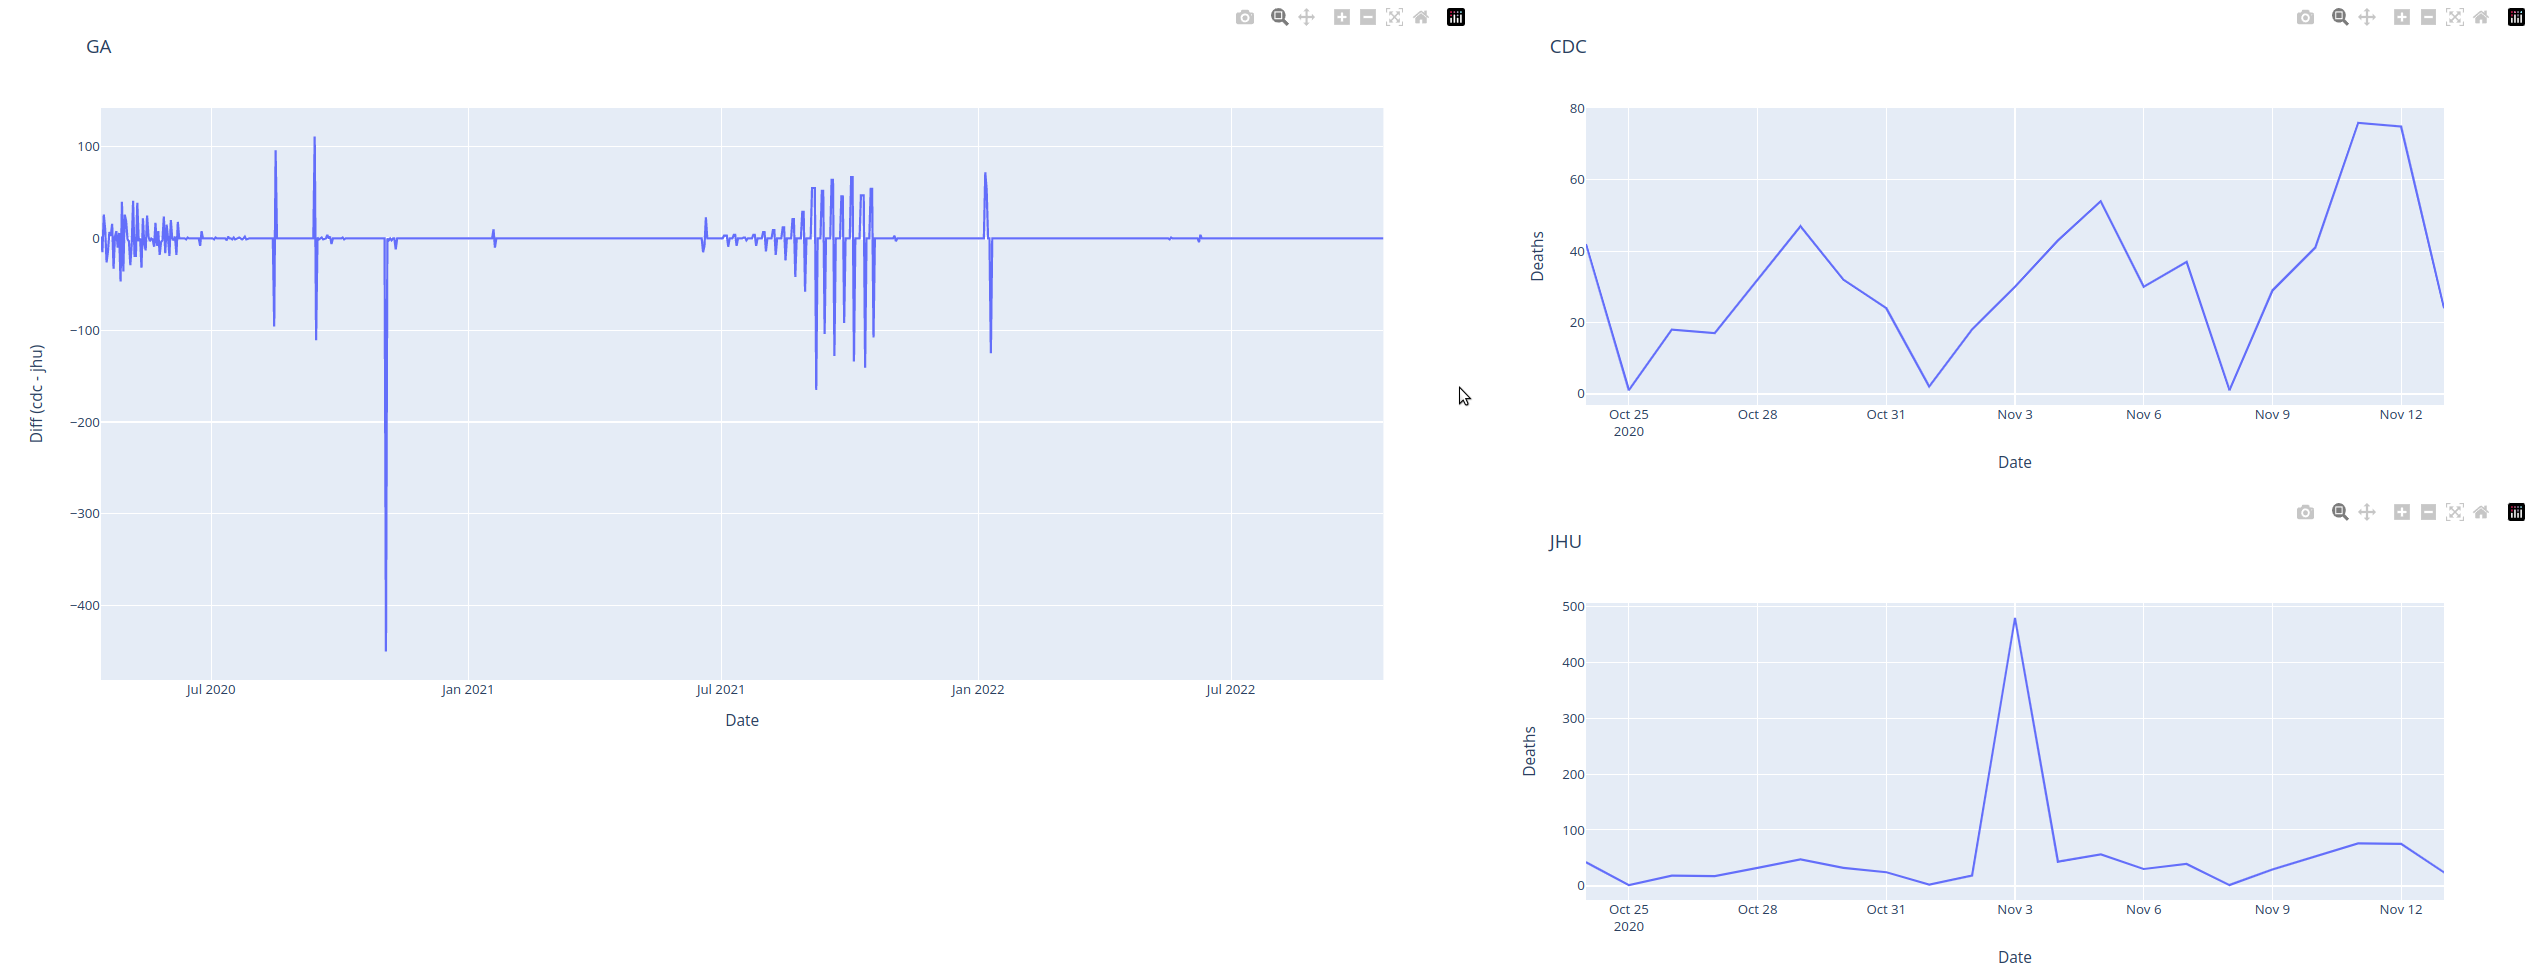
\includegraphics[width=\linewidth, height=6.3cm]{images/orig_avg_1_ga.png}
    \caption{Daily deaths in GA}
\end{subfigure}
\hfill
\begin{subfigure}{\linewidth}
    \centering
    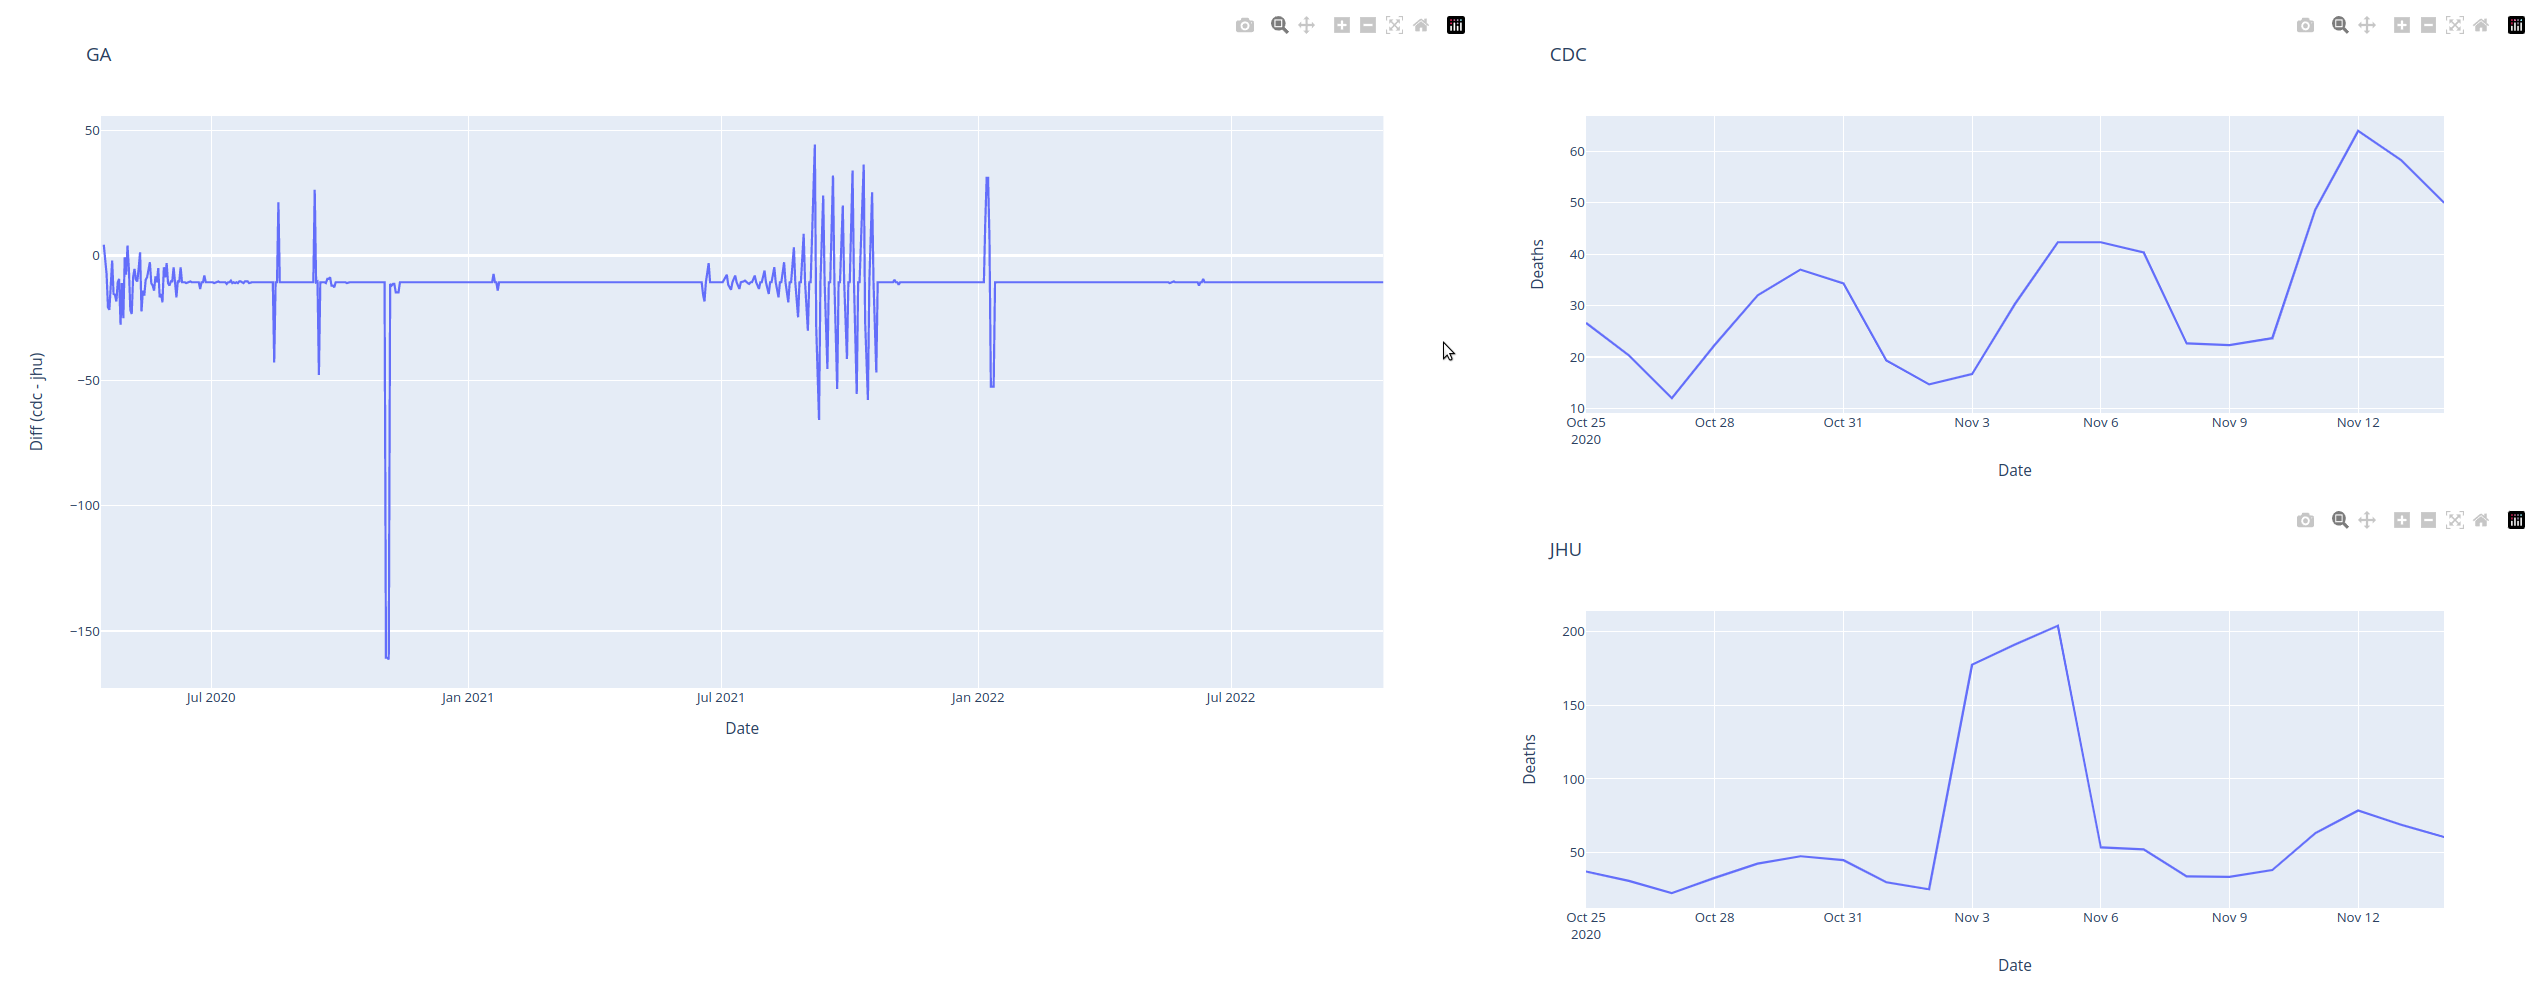
\includegraphics[width=\linewidth, height=6.3cm]{images/orig_avg_3_ga.png}
    \caption{Moving average of daily deaths with window size 3 in GA}
    \vfill
\end{subfigure}
\begin{subfigure}{\linewidth}
    \centering
    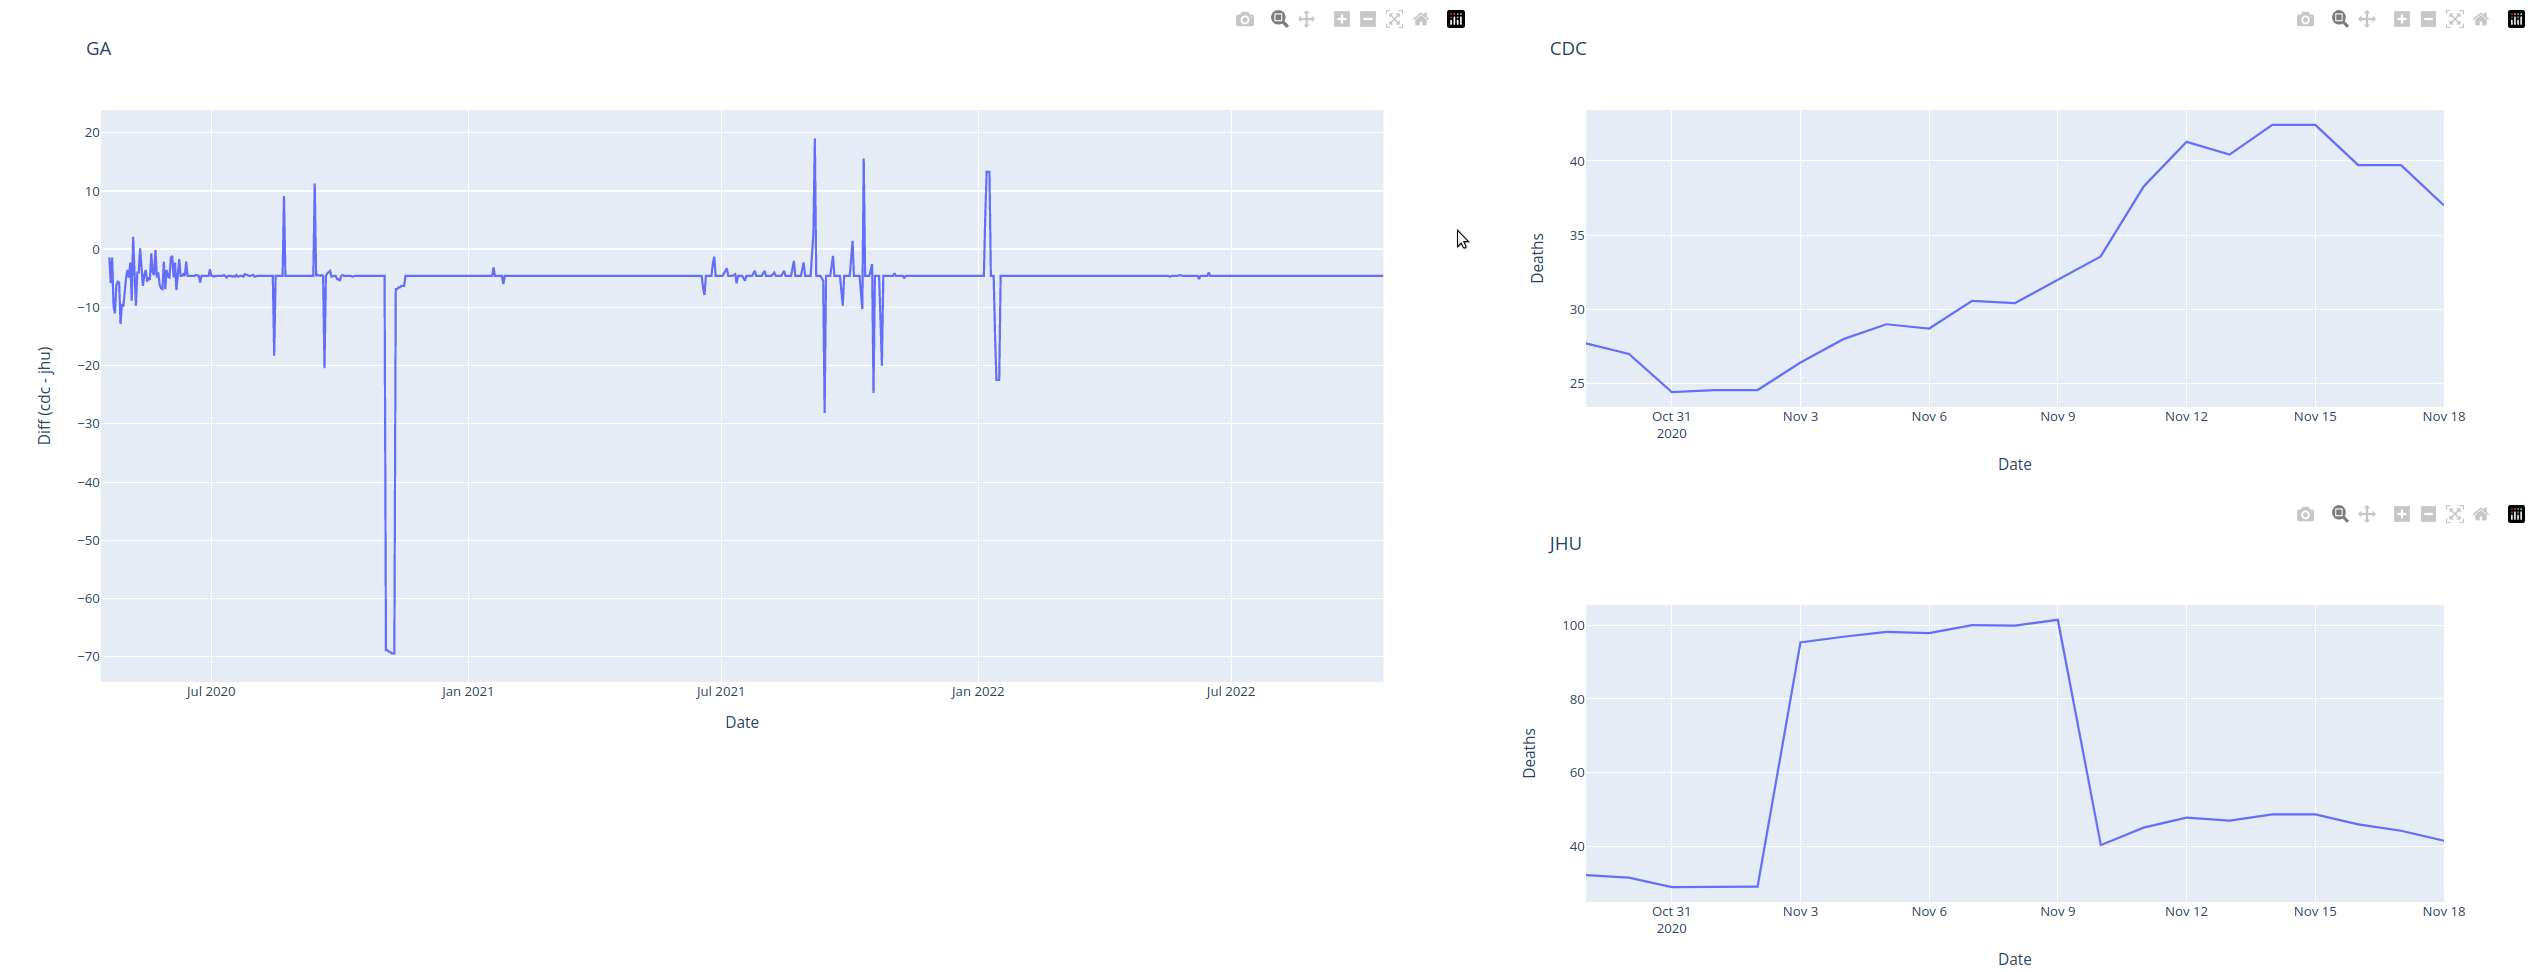
\includegraphics[width=\linewidth, height=6.3cm]{images/orig_avg_7_ga.png}
    \caption{Moving average of daily deaths with window size 7 in GA}
    \vfill
\end{subfigure}
\caption{For the top subfigure, on the left the difference between the number of deaths of CDC and JHU is shown. On top-right, CDC data is shown for the point at which the difference between CDC and JHU is maximum, with a window size of 10. On the bottom right, JHU data is shown for the point of maximum difference. Using this visualization we can easily see that there is a huge discrepancy between the number of deaths reported by CDC and JHU.}
\label{figure1}
\end{figure*}

\begin{figure*}
\centering
\begin{subfigure}{\linewidth}
    \centering
    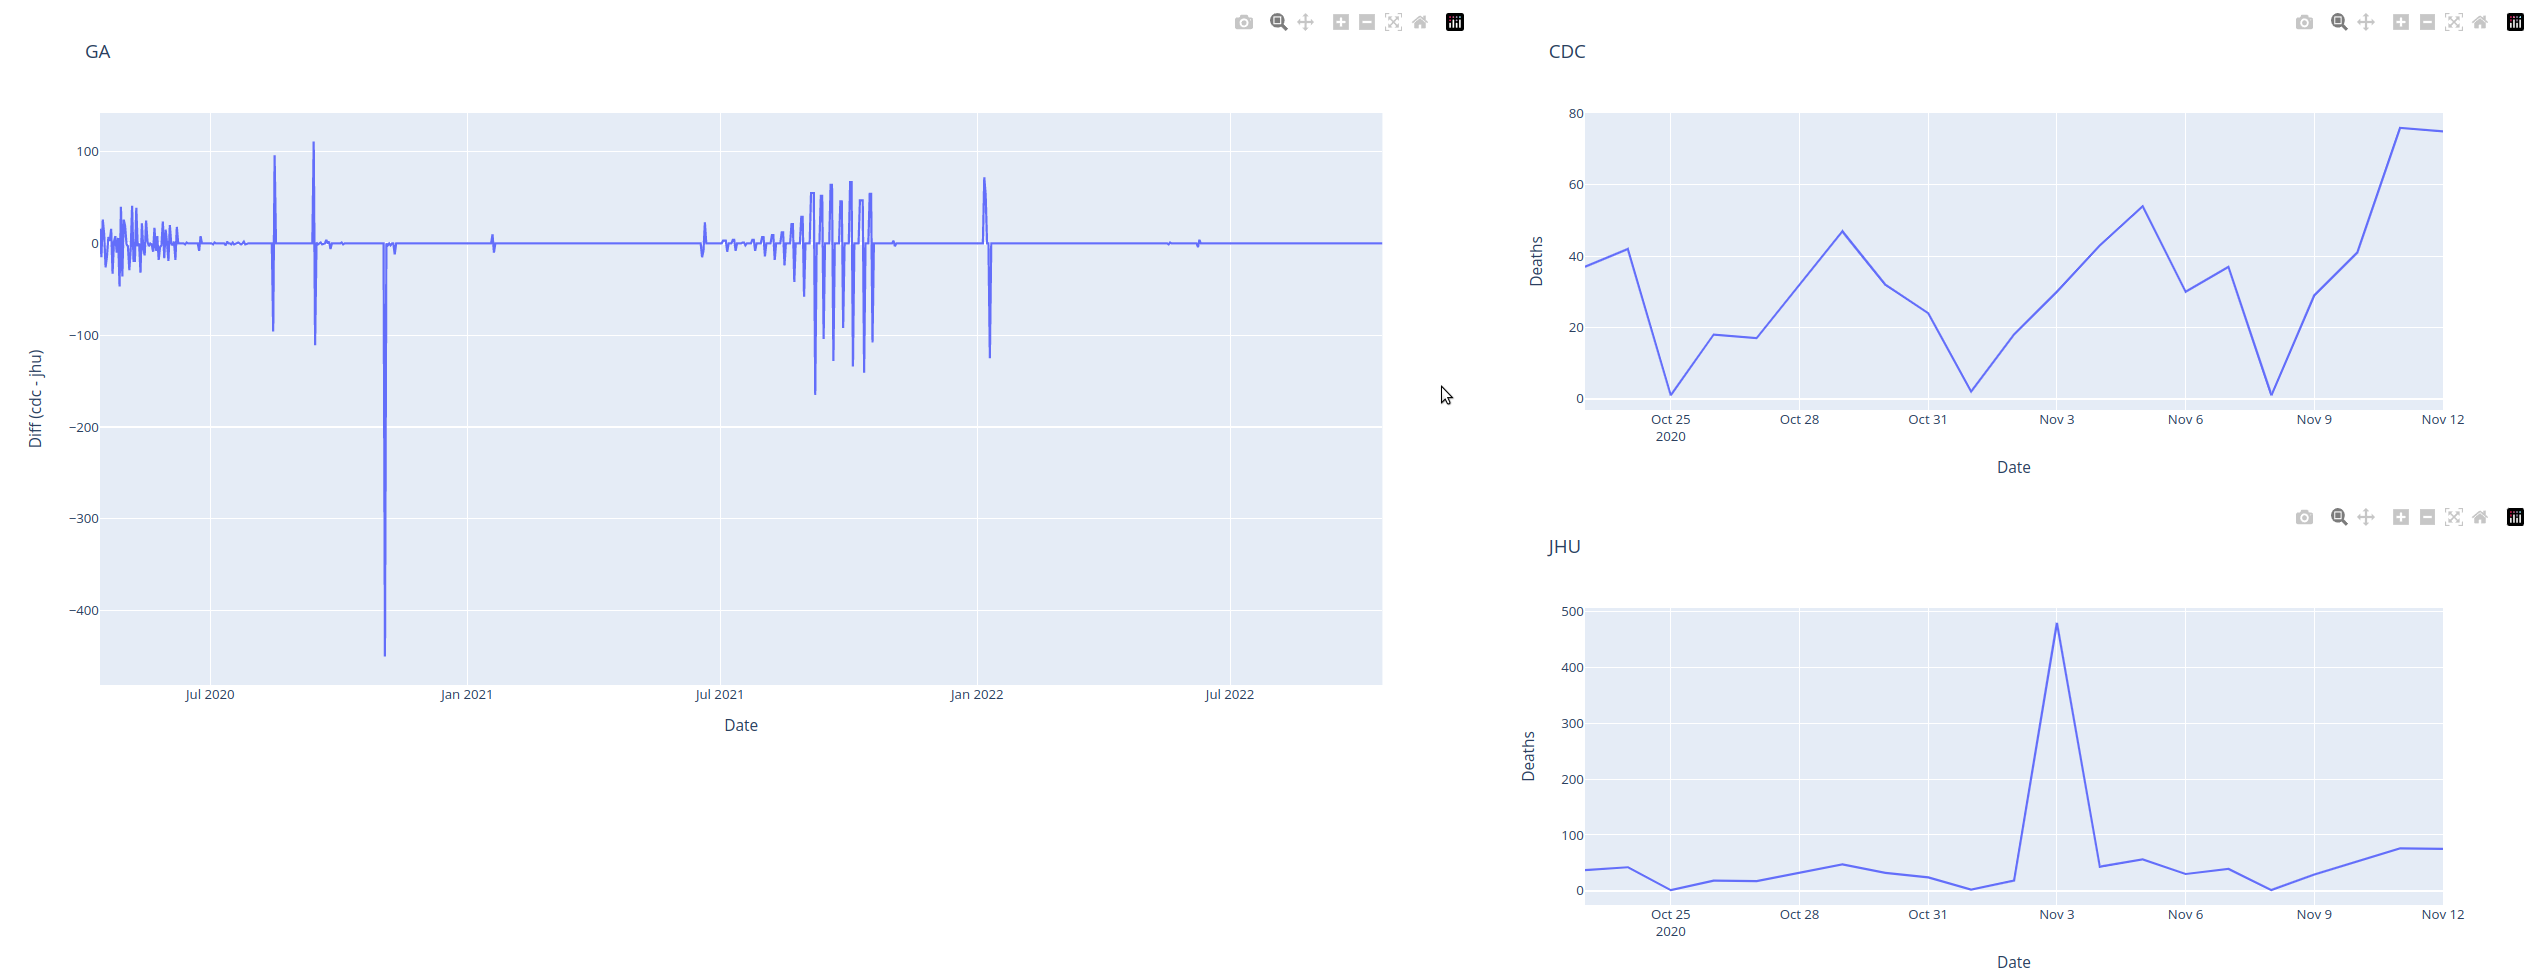
\includegraphics[width=\linewidth, height=6.3cm]{images/comb_avg_1_ga.png}
    \caption{Daily deaths in GA}
\end{subfigure}
\hfill
\begin{subfigure}{\linewidth}
    \centering
    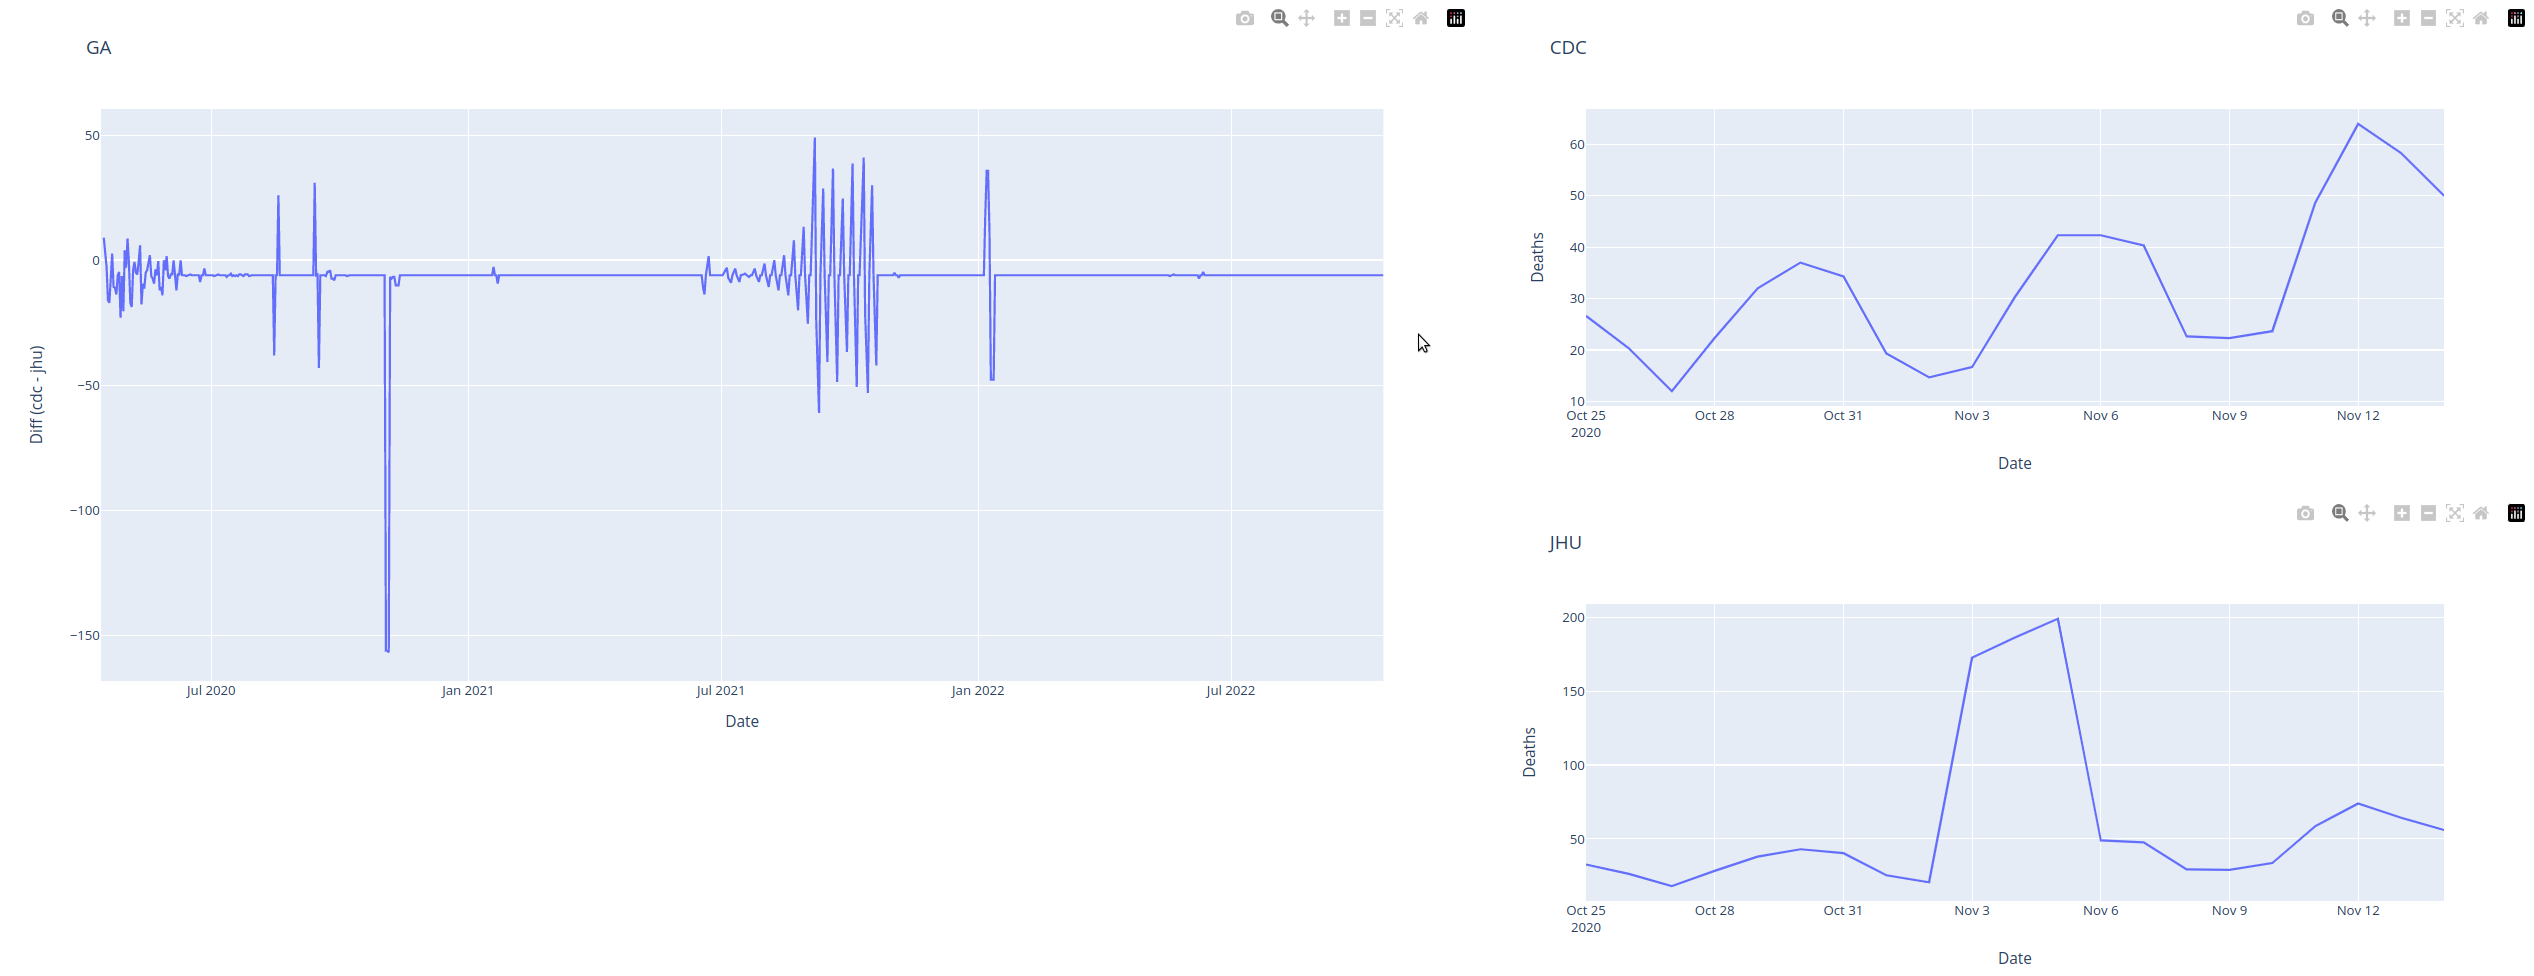
\includegraphics[width=\linewidth, height=6.3cm]{images/comb_avg_3_ga.png}
    \caption{Moving average of daily deaths with window size 3 in GA}
    \vfill
\end{subfigure}
\begin{subfigure}{\linewidth}
    \centering
    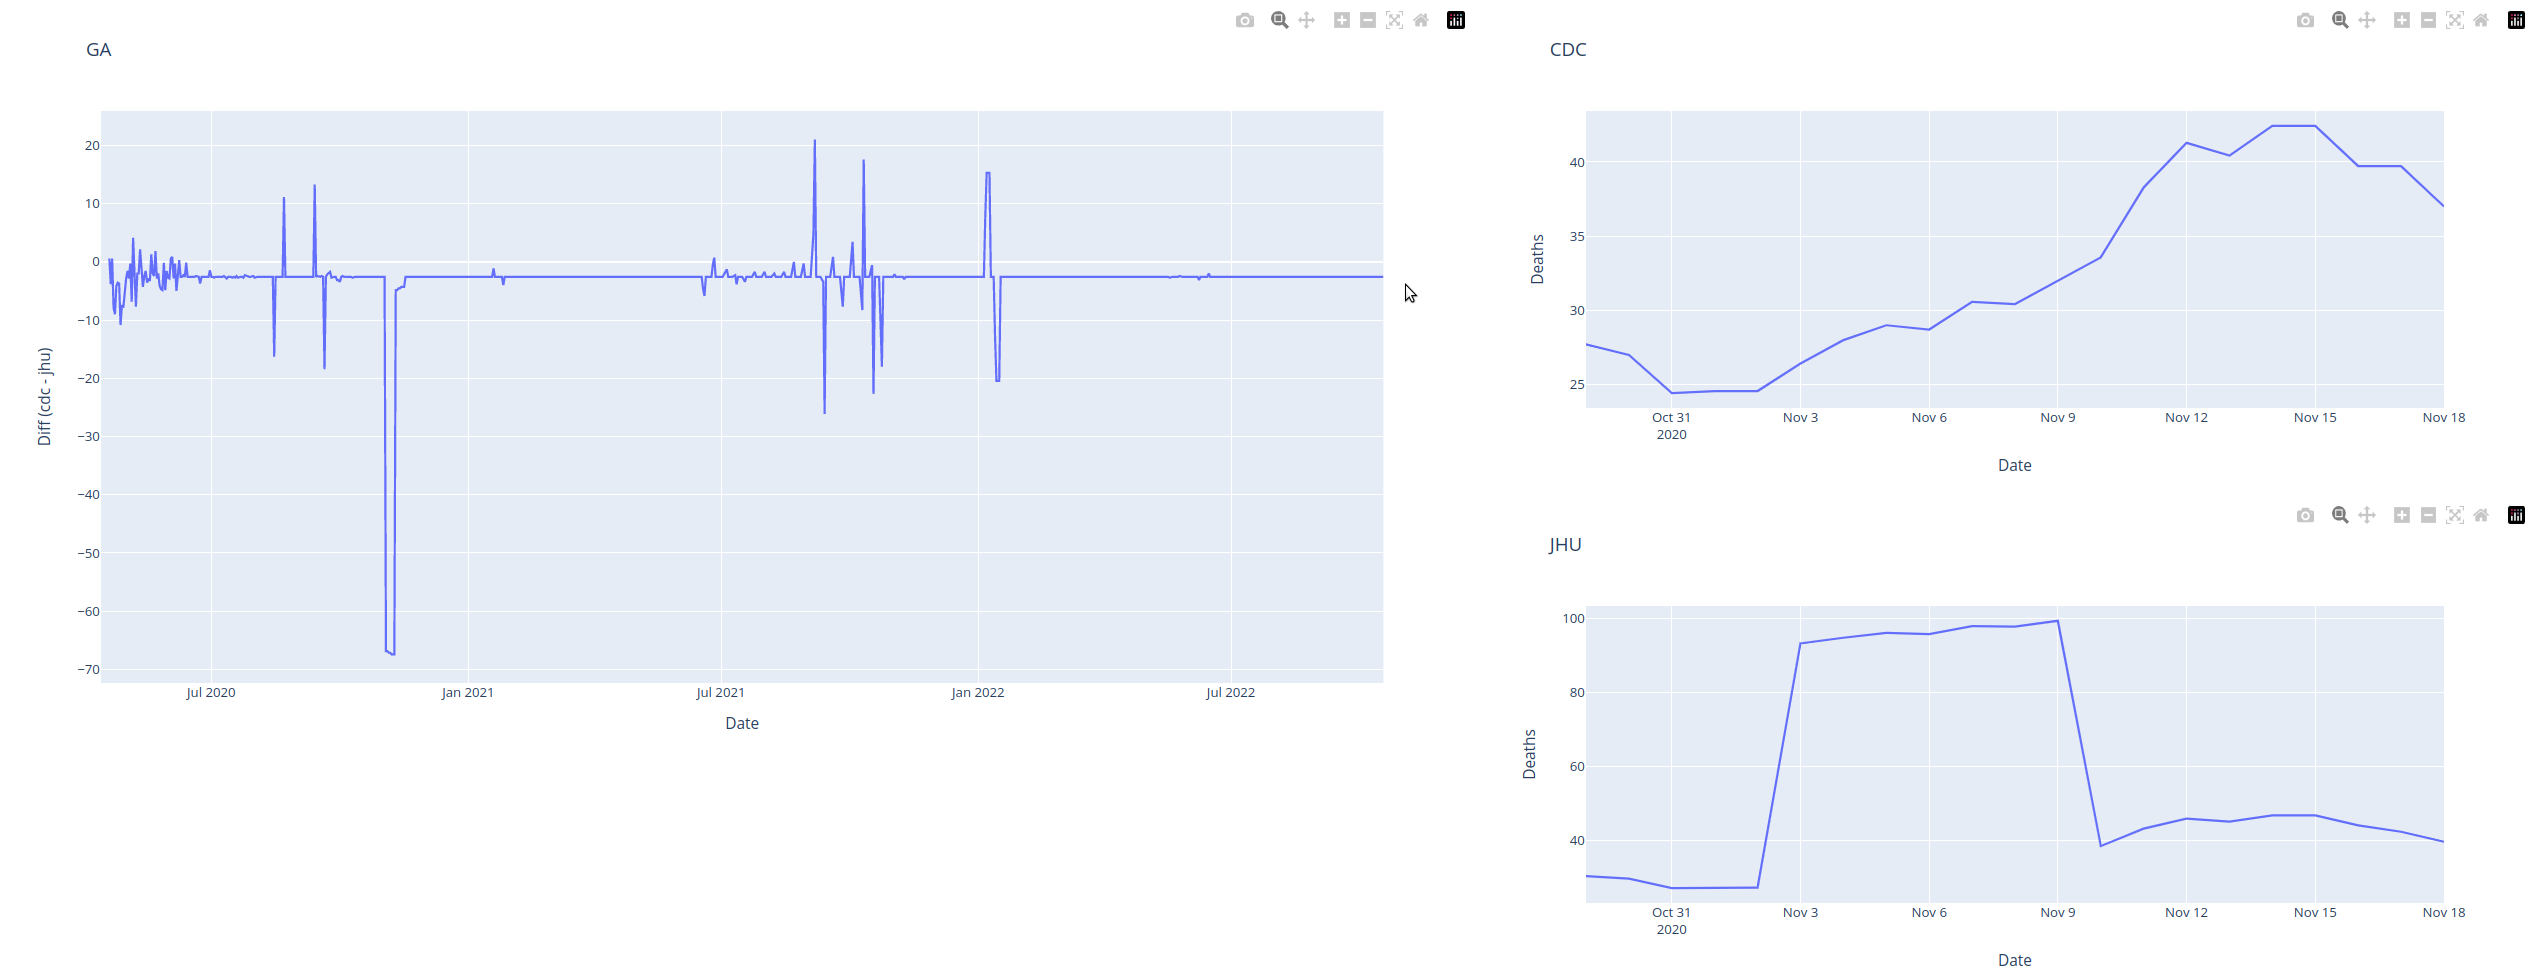
\includegraphics[width=\linewidth, height=6.3cm]{images/comb_avg_7_ga.png}
    \caption{Moving average of daily deaths with window size 7 in GA}
    \vfill
\end{subfigure}
\caption{This is similar to \cref{figure1}, except we are using the total deaths from CDC to start the JHU cumulative deaths. This is done because many papers consider CDC data to be official, and thus it makes sense to start the JHU using the value from CDC data.}
\label{figure2}
\end{figure*}

\begin{table}
    \centering
    \begin{tabular}{cc}
        \toprule
        State & Diff \\
        \midrule
        New York & 7365 \\
        Missouri & 2441 \\
        Tennessee & 2047 \\
        New Jersey & 1743 \\
        Oklahoma & 1713 \\
        Florida & 1269 \\
        \bottomrule
    \end{tabular}
    \caption{Top 6 states with the largest maximum absolute difference between the daily deaths reported by CDC and JHU.}
    \label{table2}
\end{table}

\begin{figure*}
\centering
\begin{subfigure}{0.48\linewidth}
    \begin{subfigure}{0.48\linewidth}
        \centering
        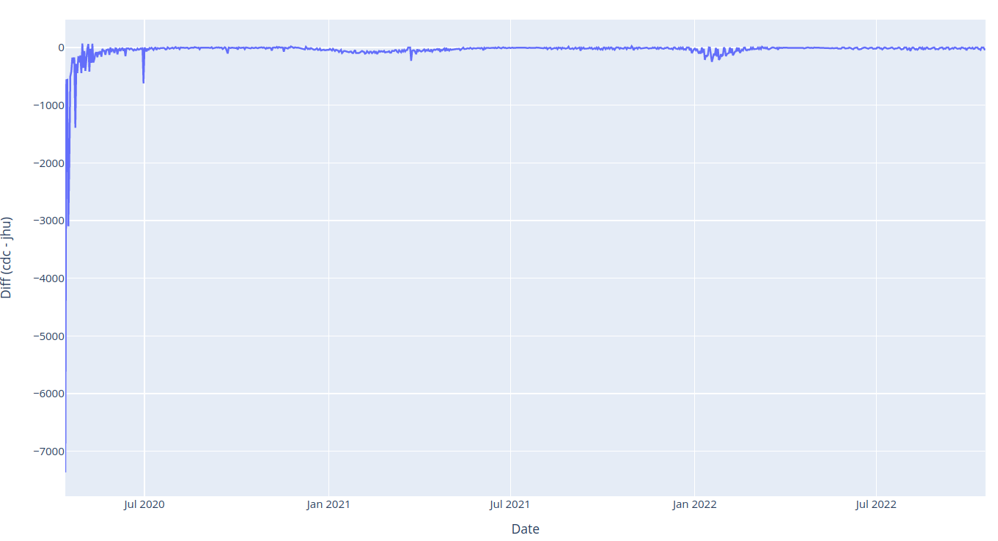
\includegraphics[width=\linewidth, height=6.3cm]{images/ny_overview.PNG}
    \end{subfigure}
    \hfill
    \begin{subfigure}{0.48\linewidth}
        \begin{subfigure}{\linewidth}
            \centering
            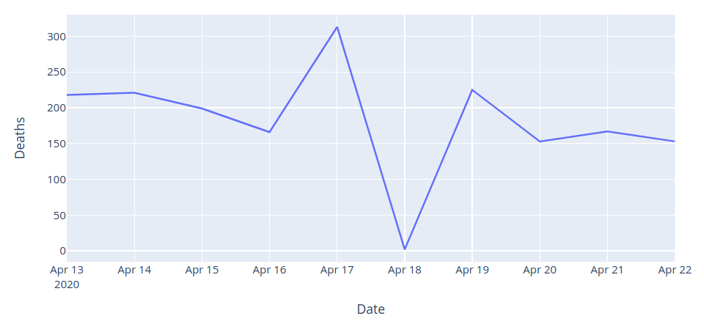
\includegraphics[width=\linewidth, height=3.15cm]{images/ny_cdc.PNG}
            \vfill
        \end{subfigure}
        \begin{subfigure}{\linewidth}
            \centering
            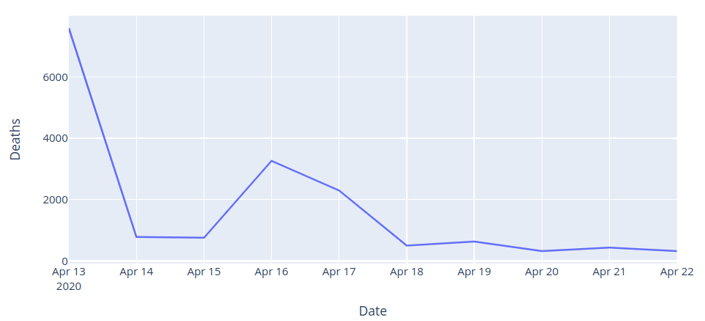
\includegraphics[width=\linewidth, height=3.15cm]{images/ny_jhu.PNG}
            \vfill
        \end{subfigure}
    \end{subfigure}
    \caption{New York}
\end{subfigure}
\hfill
\begin{subfigure}{0.48\linewidth}
    \begin{subfigure}{0.48\linewidth}
        \centering
        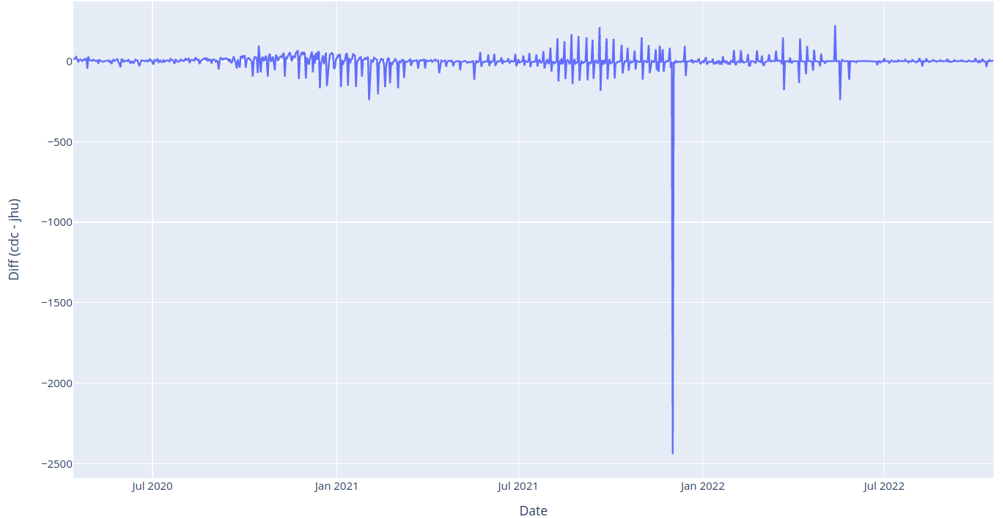
\includegraphics[width=\linewidth, height=6.3cm]{images/mo_overview.PNG}
    \end{subfigure}
    \hfill
    \begin{subfigure}{0.48\linewidth}
        \begin{subfigure}{\linewidth}
            \centering
            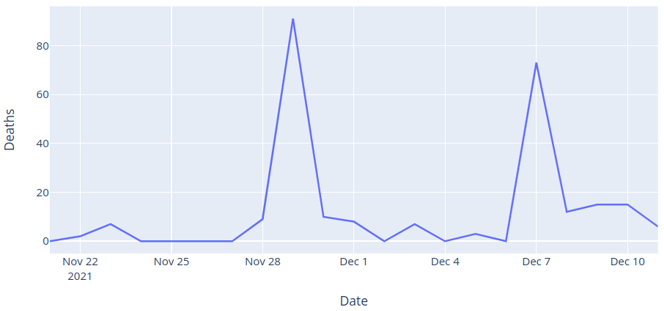
\includegraphics[width=\linewidth, height=3.15cm]{images/mo_cdc.PNG}
            \vfill
        \end{subfigure}
        \begin{subfigure}{\linewidth}
            \centering
            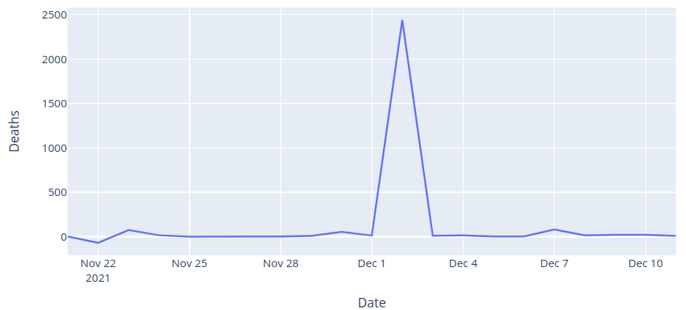
\includegraphics[width=\linewidth, height=3.15cm]{images/mo_jhu.PNG}
            \vfill
        \end{subfigure}
    \end{subfigure}
    \caption{Missouri}
\end{subfigure}
\hfill
\begin{subfigure}{0.48\linewidth}
    \begin{subfigure}{0.48\linewidth}
        \centering
        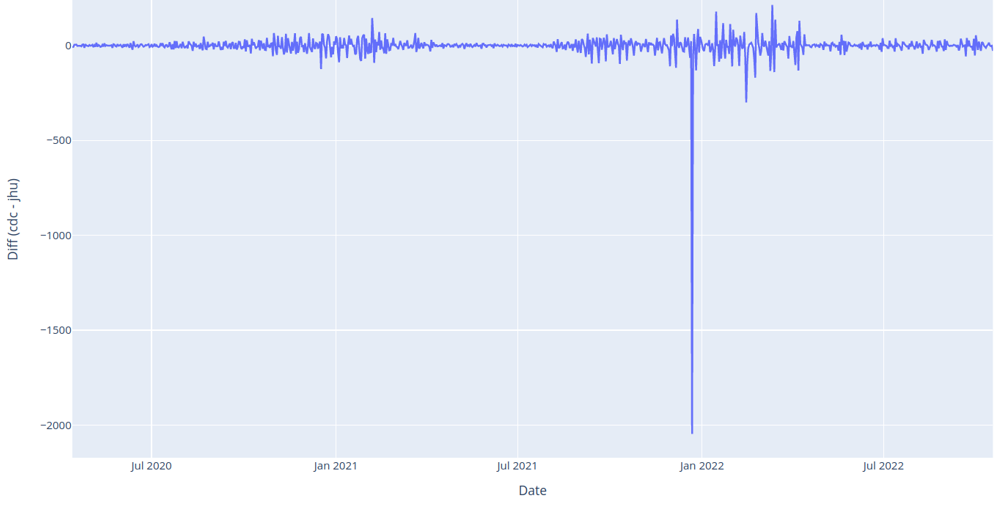
\includegraphics[width=\linewidth, height=6.3cm]{images/tn_overview.PNG}
    \end{subfigure}
    \hfill
    \begin{subfigure}{0.48\linewidth}
        \begin{subfigure}{\linewidth}
            \centering
            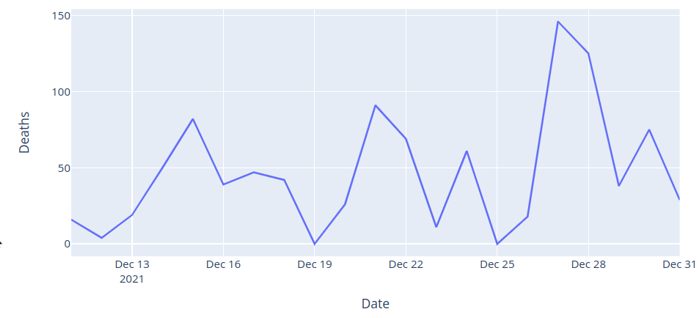
\includegraphics[width=\linewidth, height=3.15cm]{images/tn_cdc.PNG}
            \vfill
        \end{subfigure}
        \begin{subfigure}{\linewidth}
            \centering
            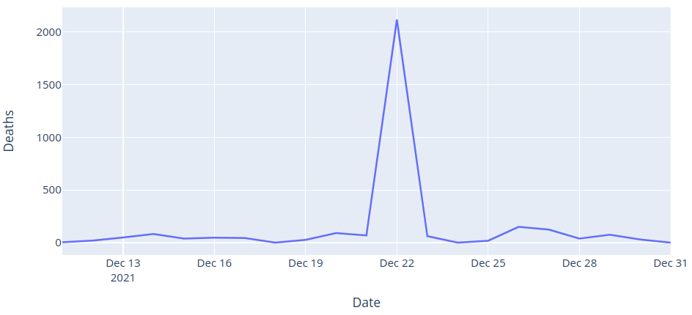
\includegraphics[width=\linewidth, height=3.15cm]{images/tn_jhu.PNG}
            \vfill
        \end{subfigure}
    \end{subfigure}
    \caption{Tennessee}
\end{subfigure}
\hfill
\begin{subfigure}{0.48\linewidth}
    \begin{subfigure}{0.48\linewidth}
        \centering
        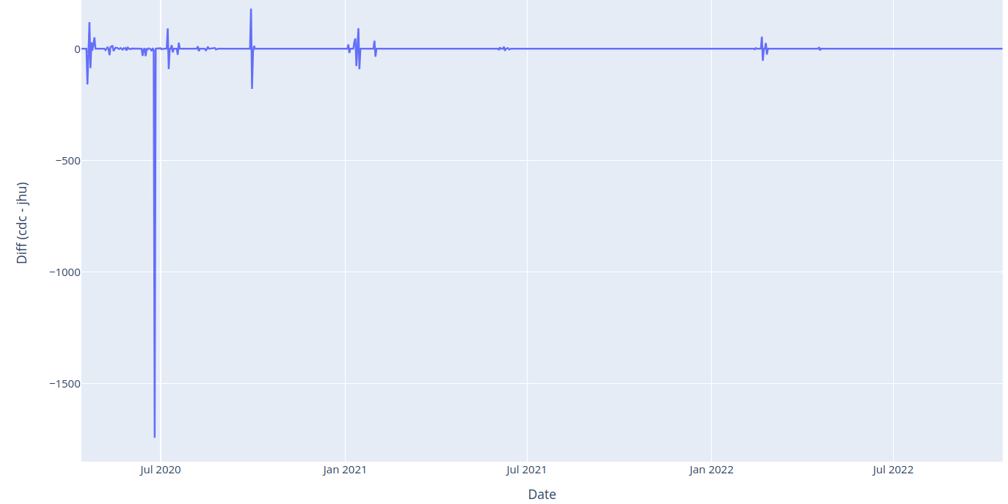
\includegraphics[width=\linewidth, height=6.3cm]{images/nj_overview.PNG}
    \end{subfigure}
    \hfill
    \begin{subfigure}{0.48\linewidth}
        \begin{subfigure}{\linewidth}
            \centering
            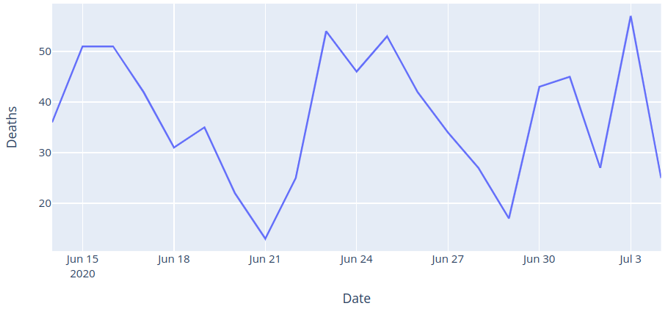
\includegraphics[width=\linewidth, height=3.15cm]{images/nj_cdc.PNG}
            \vfill
        \end{subfigure}
        \begin{subfigure}{\linewidth}
            \centering
            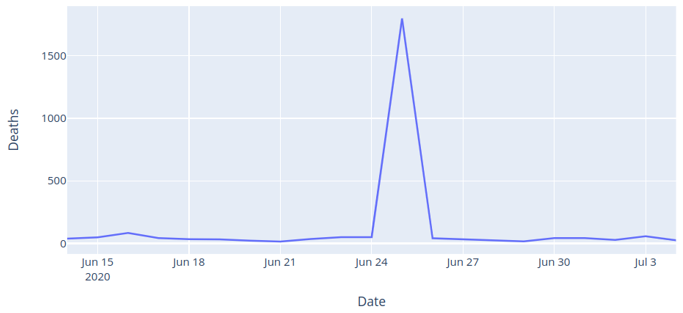
\includegraphics[width=\linewidth, height=3.15cm]{images/nj_jhu.PNG}
            \vfill
        \end{subfigure}
    \end{subfigure}
    \caption{New Jersey}
\end{subfigure}
\hfill
\begin{subfigure}{0.48\linewidth}
    \begin{subfigure}{0.48\linewidth}
        \centering
        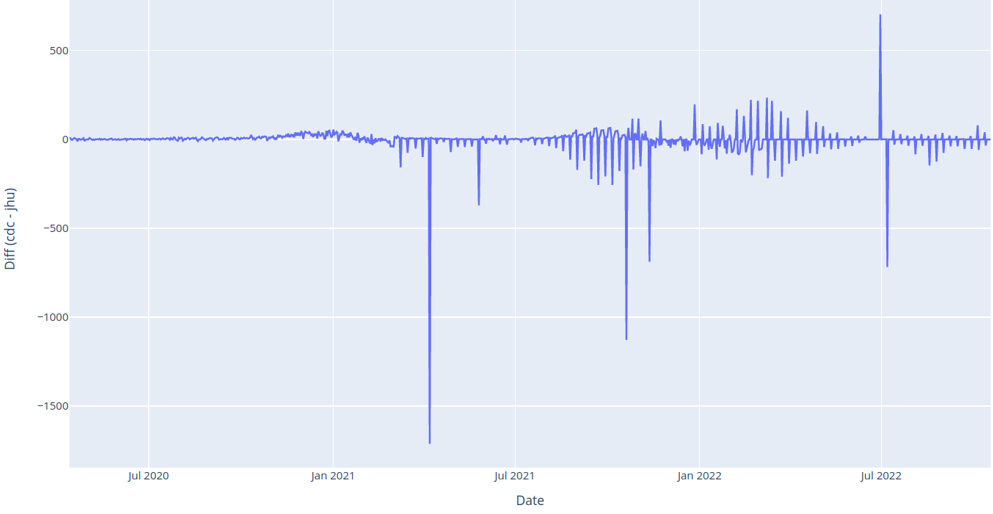
\includegraphics[width=\linewidth, height=6.3cm]{images/ok_overview.PNG}
    \end{subfigure}
    \hfill
    \begin{subfigure}{0.48\linewidth}
        \begin{subfigure}{\linewidth}
            \centering
            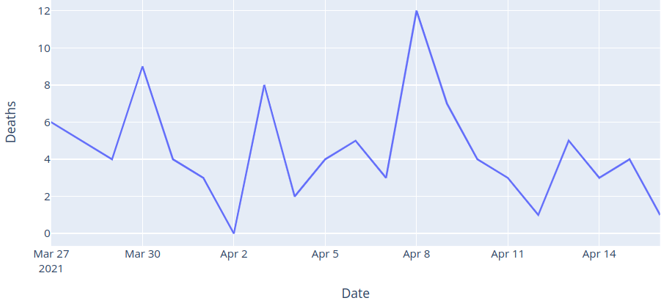
\includegraphics[width=\linewidth, height=3.15cm]{images/ok_cdc.PNG}
            \vfill
        \end{subfigure}
        \begin{subfigure}{\linewidth}
            \centering
            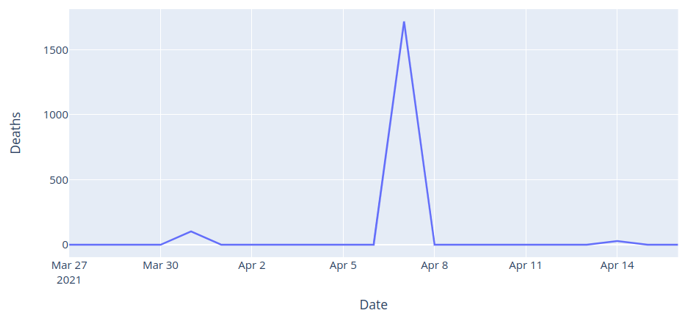
\includegraphics[width=\linewidth, height=3.15cm]{images/ok_jhu.PNG}
            \vfill
        \end{subfigure}
    \end{subfigure}
    \caption{Oklahoma}
\end{subfigure}
\hfill
\begin{subfigure}{0.48\linewidth}
    \begin{subfigure}{0.48\linewidth}
        \centering
        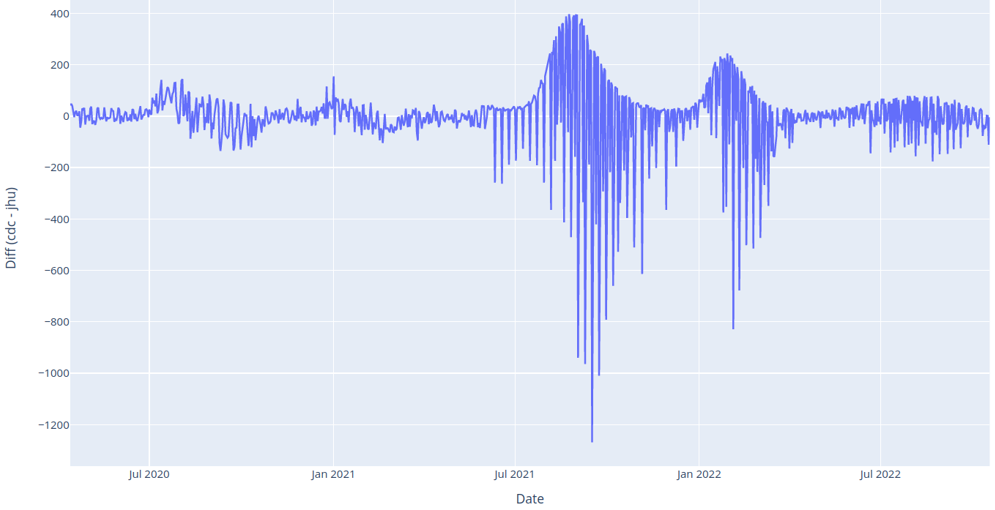
\includegraphics[width=\linewidth, height=6.3cm]{images/fl_overview.PNG}
    \end{subfigure}
    \hfill
    \begin{subfigure}{0.48\linewidth}
        \begin{subfigure}{\linewidth}
            \centering
            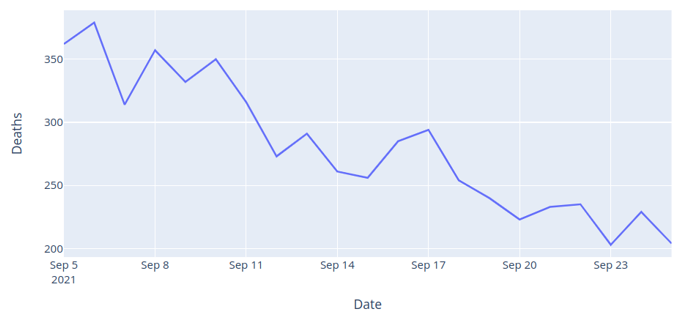
\includegraphics[width=\linewidth, height=3.15cm]{images/fl_cdc.PNG}
            \vfill
        \end{subfigure}
        \begin{subfigure}{\linewidth}
            \centering
            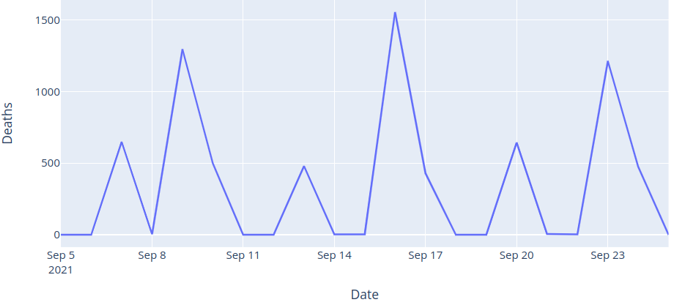
\includegraphics[width=\linewidth, height=3.15cm]{images/fl_jhu.PNG}
            \vfill
        \end{subfigure}
    \end{subfigure}
    \caption{Oklahoma}
\end{subfigure}
\caption{Similar to \cref{figure1}, the top-6 states with the largest absolute maximum difference between the reported daily deaths between CDC and JHU are shown. One pattern that emerges from these figures is that majority of these errors are caused by poor reporting by JHU data for some days, where we are able to see some cyclic patterns. Researchers trying to train machine learning models on this kind of data need to be careful, on how to deal with these outliers as these can lead to significantly poor results.}
\label{figure3}
\end{figure*}

\section{Data Quality}

Multivariate-time series models that would use the CDC or JHU data would predict the number of daily deaths for a given window in the future. But as discussed in the previous section, there are a lot of reporting errors including entering data by phone and by hand. To mitigate these issues, it is recommended that instead of using the daily deaths to train the model, using a rolling average of 7 days is much more beneficial.

To visualize the discrepancies between the daily death data of CDC and JHU, we have created a Flask app\footnote{\href{https://github.com/scalation/data/blob/master/COVID-State/data_analysis/interactive_plot.py}{COVID-State/data\_analysis/interactive\_plot.py} can be used to run 'python app.py' and it would open a web server at https://127.0.0.1:8050/} that provides an interactive visualization to see the CDC and JHU data for any date and the neighboring data with a window size of 10. You can use this tool to further visualize daily deaths, rolling averages of 3 days and 7 days.

\cref{figure1} shows the discrepancy between the CDC and JHU datasets. Here we visualize the difference between the deaths reported by CDC and JHU for the state of GA and then on the right we visualize how the CDC and JHU data look around the date with a maximum absolute difference, and as we can see the data reported by CDC and JHU is significantly different from each other. To further look into the issue, \cref{figure2} shows a similar visualization but we use the total deaths reported by CDC as the starting value for JHU total deaths. This is done because a lot of papers consider the CDC data to be ground truth and as we can see from \cref{figure2} there are still huge discrepancies between the datasets. Even using a rolling average is not sufficient to mitigate the reporting errors.

\cref{table2} shows the top-6 states with the largest absolute maximum difference between the daily deaths reported by CDC and JHU. Further looking into \cref{figure3} we can see some shocking patterns that emerge for the daily deaths reported by the CDC and JHU. We see some striking patterns in \cref{figure3} where we observe that majority of the errors are caused by poor reporting in JHU data. As we can see some significant outliers and researchers trying to train machine learning models on JHU data need to be careful about these discrepancies as it really hard to train a machine learning model that can mimic the cyclic nature as shown in the state of Florida in the JHU dataset.

\section{Conclusion}

In this paper, we looked at the quality of COVID-19 daily state data for the United State provided by two organizations CDC and JHU, which have been significantly used by researchers in the past two years to train various machine learning models for multivariate time series forecasting or for learning about the spread of the pandemic. We find that there is a significant discrepancy between the daily deaths reported by the CDC and JHU datasets. One major contributor to this discrepancy is the errors added due to humans in the loop as some portion of the data is still collected by phone or from handwritten paper. We also check for discrepancies in case we assume CDC to be the ground-truth data, and replacing the JHU total deaths with CDC total deaths for the first date still leads to similar errors. Hence, it is useful for researchers trying to train various machine learning and deep learning models for multivariate time series forecasting to be familiar with these discrepancies, as we observed that there are some patterns in the JHU dataset that appear to be very hard for a model to generalize and treating them as outliers can also be considered an option.

{\small
\bibliographystyle{ieee_fullname}
\bibliography{egbib}
}

\end{document}
